\documentclass[a4paper,12pt]{article}

\usepackage[utf8]{inputenc}
\usepackage{fullpage,url}
\usepackage{algorithm}
\usepackage{algorithmic}
\usepackage{listings}
\usepackage{amssymb,amsmath,amsthm}
\usepackage{color}
\usepackage[usenames,dvipsnames]{xcolor}
\usepackage{graphicx}

\title{Internship report at LRI}
\author{Yuto Takei \\ The University of Tokyo }

\lstset{basicstyle=\footnotesize, columns=fullflexible}
\lstdefinelanguage{Ocaml}
{
basicstyle=\ttfamily,%
morekeywords=[1]{module,sig,include,type,val,let,rec,in,begin,end,if,then,else,raise,match,try,with,exception,of,and},%
keywordstyle=[1]{\color{blue}},%
otherkeywords={},%
commentstyle=\itshape\color{Brown},%
columns=[l]fullflexible,%
sensitive=true,%
morecomment=[s]{(*}{*)},%
escapeinside={*?}{?*},%
keepspaces=true,
literate=%
{<}{$<$}{1}%
{>}{$>$}{1}%
{<=}{$\le$}{1}%
{>=}{$\ge$}{1}%
{<>}{$\ne$}{1}%
{->}{$\rightarrow$}{2}%
{<->}{$\leftrightarrow$}{2}%
}

\lstdefinelanguage{Why3}
{
basicstyle=\ttfamily,
keywordstyle=\color{blue},
morekeywords=[1]{inductive,predicate,function,goal,type,use,import,theory,end,in,axiom,lemma,export,forall,constant,module,let,exception,match,with,exists,val,for,to,while,do,done,invariant,variant},%
%keywordstyle=[1]{\color{red}},%
morekeywords=[2]{true,false},%
%keywordstyle=[2]{\color{blue}},%
otherkeywords={},%
commentstyle=\itshape\color{Brown},%
columns=[l]fullflexible,%
sensitive=true,%
morecomment=[s]{(*}{*)},%
escapeinside={*?}{?*},%
keepspaces=true,
literate=%
{v1}{v$_1$}{1}%
{v2}{v$_2$}{1}%
{v3}{v$_3$}{1}%
{n1}{n$_1$}{1}%
{n2}{n$_2$}{1}%
{d1}{d$_1$}{1}%
{d2}{d$_2$}{1}%
{<}{$<$}{1}%
{>}{$>$}{1}%
{<=}{$\le$}{1}%
{>=}{$\ge$}{1}%
{<>}{$\ne$}{1}%
{/\\}{$\land$}{1}%
{\\/}{ $\lor$ }{3}%
{\ or(}{ $\lor$(}{3}%
{not\ }{$\lnot$ }{1}%
{not(}{$\lnot$(}{1}%
{->}{$\rightarrow$}{2}%
{<->}{$\leftrightarrow$}{2}%
}

\lstnewenvironment{why3}{\lstset{language=Why3}}{}
\lstnewenvironment{ocaml}{\lstset{language=Ocaml}}{}

\newcommand{\edgen}[3]{#1\rightarrow_{#3}#2}
\newcommand{\pathn}[3]{#1\rightarrow^\star_{#3}#2}

\begin{document}

\maketitle

\begin{abstract}
  This is the abstract.
\end{abstract}

\section{Introduction}

This document reports 

\section{Contribution to ocamlgraph}

ocamlgraph \cite{conchon07tfp} is the software library for OCaml
language that provides the graph data structure and discrete
algorithms applicable on it. It also includes several implementations
of graph representation as built-in, that can be chosen in accordance
with the user's program. It is also possible to define a new data
structure optimized for specific purpose.

For example, one may want to choose the persistent graph data
implementation, any operations on which produce new instance of the
graph. On the other hand, one can also choose the imperative
implementation of graph, which addition or removal of vertex and edges
take place in the same memory location. Finally, one can arbitrarily
add the own graph implementations that satisfy the interface
requirement of ocamlgraph. The algorithms of ocamlgraph can be
performed any choice of them without any knowledge about the
implementation detail.

ocamlgraph also contains several algorithms to perform on those graph
data structure. For instance, Dijkstra's algorithm computes the
shortest path between given vertices $v_1$ and $v_2$ over any graph
with the time complexity of $O((V+E)\log(V))$. Another example is the
strongly connected component decomposition, which gives an integer
identifier to all strongly connected components and returns the
mapping from vertex to the identifier which the vertex belongs to.

\subsection {Implementation of the Bellman-Ford algorithm}

During the internship, I contributed to the enrichment of the
algorithms of ocamlgraph, and added the implementation of Bellman-Ford
algorithm. It is the algorithm that also computes the shortest path
from $v_1$ to $v_2$, but allows the graph to have a negative weight on
the edge unlike the Dijkstra's algorithm. After the termination, it
gives a mapping from every vertex $v$ to the integer representing the
shortest path distance from given $s$ to every $v$. In case that the
graph contains a negative length cycle, the edges in which sum up to
below zero, the algorithm reports the existence of such the cycle.

First I briefly describe the mechanism of the algorithm according to
the literature \cite{algo}. It maintains the labels that are given on
every node in graph $G$. The label is represented as the pair
$(\pi,d)$ for every node $v$, respectively denoting the predecessor in
the shortest path tree, and the shortest path distance from $s$ after
algorithm termination. It is first initialized as $(nil,\infty)$ for
all nodes except $s$ having $(nil,0)$. Algorithm \ref{alg:init} shows
the operation.

\newcommand{\initBF}{\ensuremath{\mbox{\sc Initialize-Single-Source}}}
\begin{algorithm}
\caption{$\initBF(G,s)$}\label{alg:init}
\begin{algorithmic}[1]
\FORALL{vertex $v\in V[G]$}
\STATE{$d[v]\leftarrow\infty$}
\STATE{$\pi[v]\leftarrow nil$}
\ENDFOR
\STATE{$d[s]\leftarrow 0$}
\end{algorithmic}
\end{algorithm}

The fundamental part of the algorithm is to make use of every edges to
improve the distance given for vertices. This operation is called
relax, as shown in Algorithm \ref{alg:relax}. It tests $(u,v)$ is
interesting for reducing the known distance from $s$ to $v$ at the
moment of execution.

\newcommand{\relaxBF}{\ensuremath{\mbox{\sc Relax}}}
\begin{algorithm}
\caption{$\relaxBF(u,v,l)$}\label{alg:relax}
\begin{algorithmic}[1]
\IF{$d[v]>d[u]+l(u,v)$}
\STATE{$d[v]\leftarrow d[u]+l(u,v)$}
\STATE{$\pi[v]\leftarrow u$}
\ENDIF
\end{algorithmic}
\end{algorithm}

Finally, we show the complete psuedo-code for the Bellman-Ford
algorithm in Algorithm \ref{alg:bf}. We firstly initialize the labels
by \initBF, and iterate \relaxBF over all edges for $|V|-1$ times.

This upper bound is given according to the maximum possible depth of
the shortest path tree. For the relation to the next section, I show
an informal proof on it. Note that the vertex whose shortest path has
$n$ steps from $s$ will acquire the shortest distance after $n$-th
iteration. Because any shortest path tree have less than $|V|-1$
depths, it is suffice to iterate relaxation for that number;
otherwise, suppose the shortest path $p=[v_1;v_2;...;v_n]$ exists for
$n>|V|-1$ and there must exists such $i,j$ that $i\ne j$ and $v_i=v_j$
according to the pigeon hole principal. However, if the length of the
loop $[v_i;v_{i+1};...;v_j]$ is positive, we can make a shorter path
$p'=[v_1;v_2;...;v_{i-1};v_i;v_{j+1};...;v_n]$ than $p$ by contracting
the loop. Otherwise when the length is negative, we can make
artbitrarily shorter path by repeating the loop. Thus in either way,
the shortest assumption of $p$ leads to the contradiction. If the
length is zero, contracted loop $p'$ has smaller number of
intermediate vertices and thus we can eventually acquire the path less
than $|V|$ steps by induction.

In such a case that the negative length cycle exists in $G$, one can
perform \relaxBF infinitely, gaining arbitrarily small number for its
distance as stated above. Therefore, the loop from line 7-11 tests if
there exists an edge still to be relaxed. If the algorithm does not
detect any negative length cycle, it returns True for the indication.

The time complexity of this algorithm is $O(|E|\cdot|V|)$.

\newcommand{\mainBF}{\ensuremath{\mbox{\sc Bellman-Ford}}}
\begin{algorithm}
\caption{$\mainBF(G,s,l)$}\label{alg:bf}
\begin{algorithmic}[1]
\STATE{$\initBF(G,s)$}
\FOR{$i=1\to|V[G]|-1$}
\FORALL{edge $(u,v)\in E[G]$}
\STATE{$\relaxBF(u,v,l)$}
\ENDFOR
\ENDFOR
\FORALL{edge $(u,v)\in E[G]$}
\IF{$d[v]>d[u]+l(u,v)$}
\RETURN{False}
\ENDIF
\ENDFOR
\RETURN{True}
\end{algorithmic}
\end{algorithm}

For the purporse of the implementation for ocamlgraph, my
implementation is provided as a functor that receives the module type
for graph and weigt on every edge. Making use of the record
polymorphism in OCaml language, I introduced the minimum definition of
graph data structure that the algorithm requires (Listing
\ref{lst:graph}).

\floatname{algorithm}{Listing}
\setcounter{algorithm}{0}
\begin{algorithm}
\caption{Minimum required interface of the graph}\label{lst:graph}
\begin{ocaml}
module type G = sig
  type t
  module V : Sig.COMPARABLE
  module E : sig
    type t
    type label
    val label : t -> label
    val src : t -> V.t
    val dst : t -> V.t
  end
  val fold_edges_e : (E.t -> 'a -> 'a) -> t -> 'a -> 'a
  val nb_vertex : t -> int
end
\end{ocaml}
\end{algorithm}

This means that the graph data structure should provide a function
that returns the number of edges (to compute $|V|-1$) and one that
provides the way to execute fold operation over all edges in the
graph. This is required to perform relaxation for all edges, and at
the same time, to check if relaxation happened on at least one
edge. When the graph reaches to the stable state, i.e. no any relaxion
occurs anymore, one can exit the relaxation loop before reaches to the
terminal. In most cases, this largely contributes to the optimization
of the algorithm.

As for the weight for edges, it is given as in Listing
\ref{lst:weight}. The weight can be any type that is a monoid with
total order.

\begin{algorithm}
\caption{Minimum definition of the weight}\label{lst:weight}
\begin{ocaml}
module type WEIGHT = sig
  type label
  type t
  val weight : label -> t
  val compare : t -> t -> int
  val add : t -> t -> t
  val zero : t
end
\end{ocaml}
\end{algorithm}

By making use of \texttt{G} and \texttt{WEIGHT} module type, I now
introduce the functor signature for Bellman-Ford algorithm in Listing
\ref{lst:bfsig}. The pair of \texttt{G} and \texttt{WEIGHT} expresses
weighted directed graph. The algorithm is instanciated by receiving it
as a functor parameter.

\begin{algorithm}
\caption{Module interface of Bellman-Ford algorithm}\label{lst:bfsig}
\begin{ocaml}
module BellmanFord
  (G: G)
  (W: WEIGHT with type label = G.E.label) :
sig
  module H : Hashtbl.S with type key = G.V.t

  exception Negative_cycle of G.E.t list

  val all_shortest_paths : G.t -> G.V.t -> W.t H.t
  val find_negative_cycle_from: G.t -> G.V.t -> G.E.t list
  val find_negative_cycle: G.t -> G.E.t list
end
\end{ocaml}
\end{algorithm}

I implemented three methods in this module as listed below.

\begin{itemize}
\item \texttt{all\_shortest\_paths} receives a graph $G$ and the
  source vertex $s\in V$, and returns a hashtable which maps a vertex
  $v\in V$ to the total weight of the shortest path from $s$ to
  $v$. When there exists a negative length cycle, it raises an
  exception.

\item \texttt{find\_negative\_cycle\_from} also receives $G$ and $s$,
  and looks for a negative length cycle reachable from $s$. When
  found, it returns a list of edges that involve in such a
  cycle. Otherwise, it raises an exception.

\item \texttt{find\_negative\_cycle} receives only $G$. It looks for
  any negative cycle in the graph, and when found, returns one of
  them. Otherwise, it raises an exception.
\end{itemize}

The first two methods works as just the same except for the opposite
behavior on raising exception.  They are both provided for the
convenience of ocamlgraph users.

The last method \texttt{find\_negative\_cycle} is slightly more
complex. It decompose the graph into strongly connected components,
and perform \texttt{find\_negative\_cycle\_from} from one of the
vertex in each components. In this way, we can traverse the graph to
all vertices without giving such a vertex as $s$.

However, this implementation is very naive and there is a room for
improvement. For example, just look for the cycle in each strongly
connected component is sufficient for this purpose. This can reduce
$|E|$ and $|V|$ in time complexity, enabling the faster execution of
the method.

The optimization for this method is left for the future work.

\subsection{Incremental graph builder without negative length cycle}

As stated in the first, ocamlgraph allows users to implement any
arbitrarily data structure that goes along the built-in algorithms. So
as for the other contribution on ocamlgraph library, I added the new
graph implementation that ensures the graph is free of negative length
cycle. This graph module helps users to immediately find such a cycle
and prevent some algorithms from being unable to compute the result
(e.g. shortest paths).

Listing \ref{lst:nng} shows the functor signature for persistent graph
data structure. Similar to the module BellmanFord, it receives the
graph and weight module types. Note that \texttt{Sig.P} is the module
type that encapsulate the persistent graph data structure. This
functor returns the module that include all operations applicable on
\texttt{Sig.P}.

\begin{algorithm}
\caption{Signature for persistent graph without negative length cycle}\label{lst:nng}
\begin{ocaml}
module Persistent
  (G: Sig.P)
  (W: WEIGHT with type label = G.E.label) :
sig
  include Sig.P with module V = G.V and module E = G.E

  exception Negative_cycle of G.E.t list
end
\end{ocaml}
\end{algorithm}

Additionally, as the main feature of this module, it raises
\texttt{Negative\_cycle} exception whenever the user operation is
about to introduce a negative length cycle. As a result, such
operation is prohibited over this graph.

The implementation of this graph $G$ involves in maintaining the set
of top ancestors in the graph, and distances from them to all
nodes. Let $S$ denote the set of ancestors and $d[s\to v]$ denote the
shortest path distance from $s\in S$ to $v\in V$. When $[v]_G$ denotes
the set of vertices that are strongly connected with $v$ in $G$, any
$s\in S$ should not be reachable from $V\backslash[s]_G$. Also if
$s\in S$, $\forall v\in[s]_G\backslash\{s\}; v\notin S$. Finally, any
vertex $v\in V$ has at least one $s\in S$ such that $s$ is the
ancestor of $v$. Intuitionally, this keeps $S$ to be the minimum set
of ancestor vertices that all vertices are reachable from at least one
vertex in $S$.

When one adds a new vertex $v$ to $G$, $v$ cannnot be reached from any
vertex in $S$, we should update as $S\leftarrow S\cup\{v\}$. At this
moment, we also set $d[v\to v]\leftarrow 0$, and for other vertices
$x$, set $d[v\to x]\leftarrow \infty$. (see Algorithm
\ref{alg:verNng})

\floatname{algorithm}{Algorithm}
\setcounter{algorithm}{3}
\begin{algorithm}
\caption{$\ensuremath{\mbox{\sc Add-Vertex}}(G,S,d,v)$}\label{alg:verNng}
\begin{algorithmic}[1]
\STATE{$G'\leftarrow$ Add $v$ to $G$}
\STATE{$S'\leftarrow S\cup\{v\}$}
\STATE{$d'\leftarrow d\cup\{v\to x:\infty,v\to v:0\}$}
\RETURN{$(G',S',d')$}
\end{algorithmic}
\end{algorithm}

When one adds a new edge $(u,v)$ to $G$, we need to update the
distance mapping $d$, so that it correctly keeps the shortest path
distance. However before that, if $v\in S$, we should determine
whether to keep $v$ in $S$ or not. In order to preserve the property
above, we should know $u$ becomes an predecessor to $v$ or $u$ remains
in the same strongly connected component, which can be known by
counting how many vertices in $S$ can reach $u$ in $G$. (see Algorithm
\ref{alg:edgNng})

After appropriately updating $S$, start to update $d$ for descendants
of $v$. This can be done by relax operations of the edges with
improved version of Bellman-Ford algorithm, which utilizes a queue to
manage the order of edge relaxation. During the relax operations, if one
reaches back to $u$, this means $(u, v)$ introduced a negative cycle.

\begin{algorithm}
\caption{$\ensuremath{\mbox{\sc Add-Edge}}(G,S,d,u,v)$}\label{alg:edgNng}
\begin{algorithmic}[1]
\STATE{$G\leftarrow$ Add $(u,v)$ to $G$}
\IF{$v\in S$}
\STATE{$n\leftarrow\{s\in S\vert d[s\to u]\ne \infty\}$}
\IF{$n\ne\{v\}$}
\STATE{$S\leftarrow S\slash\{v\}$}
\STATE{$d\leftarrow d\cup\{v\to x:\infty\}$}
\ENDIF
\ENDIF
\STATE{$d\leftarrow Relax(G,u,v,d)$}
\RETURN{$(G,S,d)$}
\end{algorithmic}
\end{algorithm}

As for the removal of either vertex or edge, because it costs ver much
to calculate the distance mapping after removal, my implementation
chose to reconstruct the distance mapping table by using $S$.

\section{Formal proofs of Bellman-Ford algorithm on Why3}

Why3 \cite{boogie11why3} is a software verification platfrom that
enables one to describe the algorithm properties by first-order
logic. One of its important features is the ability to separate the
logical statements from programs.

Logic component is described by set of theories that contains the
definition of data types, their characteristics as either an axiom or
a lemma, and predicates (or functions if returns non-Boolean) upon the
given arguments. On the other hand, program component takes over the
similar syntax as OCaml, but we additionally define conditions of the
program by means of Hoare Logic.

Another advantage in using Why3 is the ability to prove the goal by
combining several different SMT provers. Why3 recognizes the goals to
solve in the course of verification and provides a way to split into
smaller goals. Those smaller goals are then transformed into several
formats so that different SMT provers can try to solve them.

During my latter half of the internship, I devoted myself to proving
the correctness of Bellman-Ford algorithm by using Why3.

\subsection{Specification}

Proving the algorithm first starts by providing the specification of
the algorithm. It should be minimal yet comprehensive to define the
behavior of algorithm and should be clearly distinguished from the
proofs. First, shown below in Listing \ref{lst:why3graph} is a
definition of graph representation that I used for proving
Bellman-Ford algorithm.

\floatname{algorithm}{Listing}
\setcounter{algorithm}{4}
\begin{algorithm}
\caption{Graph representation in Why3 syntax}\label{lst:why3graph}
\begin{why3}
theory Graph
  use export set.Fset (* theory concerning finite sets *)

  type vertex
  constant vertices : set vertex
  constant edges: set (vertex, vertex)
  function weight vertex vertex : int

  constant s : vertex (* source vertex *)
  axiom s_in_graph: mem s vertices

  axiom edges_def:
    forall x y: vertex. mem (x, y) edges ->
    (mem x vertices /\ mem y vertices)
end
\end{why3}
\end{algorithm}

\texttt{Graph} is a theory that encapsulates the all logical
characteristics of my graph data structure. As you can easily
understand, it defines \texttt{vertex} type for the vertex
representation, and \texttt{vertices} and \texttt{edges} provide
storage of actual graph structure. However, in the proof, their solid
values are never to be determined and instead, assumed to take all
possible values that satisfy other constraints. For example, due to
the axiom \texttt{s\_in\_graph}, \texttt{s} can take any one element
in \texttt{vertices}. In the same way, \texttt{edges\_def} restricts
any element in \texttt{edges} should be a pair of elements that both
belongs to \texttt{vertices}. As a whole, \texttt{Graph} has an
ability to express any graph for the algorithm.

For the next, having the definition of the graph, I define the
interface of the algorithm. In this case, it is needed to slightly
modify the structure from the pusedo-code that was introduced in the
earlier section. Because we already have the interface to access the
graph structure defined previously, we can omit graph-related
parameters for simplicity. As a result, the algorithm now receives
nothing and returns a mapping from each vertex to the shortest path
distance. Note that for the purpose to handle $\infty$ as a distance
value, an algebraic datatype \texttt{dist} is defined. By using it,
the return type of the algorithm can be then expressed as \texttt{map
  vertex dist} as in Listing \ref{lst:why3int}. In case the algorithm
detects a negative cycle, it raises \texttt{Negative\_cycle}
exception.

\begin{algorithm}
\caption{Interface definition of Bellman-Ford algorithm}\label{lst:why3int}
\begin{why3}
type dist = Finite int | Infinite
exception Negative_cycle
val bellman_ford : unit -> map vertex dist
\end{why3}
\end{algorithm}

Given the structure of the graph, I then introduce the notion of the
path between two vertices, shown in Listing \ref{lst:why3path}. The
predicate \texttt{path u v n d} means that the path of \texttt{d}
steps exists from \texttt{u} to \texttt{v} with \texttt{n} length. It
is inductively defined; the empty case is that all the vertices can
reach themselves without any step, thus no length. Then as a successor
case, path from \texttt{u} to \texttt{v} is extended by using an edge
from \texttt{v} to \texttt{w}, becoming a path from \texttt{u} to
\texttt{w}.

\begin{algorithm}
\caption{Difinition of path}\label{lst:why3path}
\begin{why3}
theory Path
  use import Graph

  inductive path vertex vertex int int =
    | path_empty:
        forall v: vertex. path v v 0 0
    | path_succ:
        forall v1 v2: vertex, n d: int. path v1 v2 n d ->
        forall v3: vertex. mem (v2, v3) edges ->
        path v1 v3 (n + (weight v2 v3)) (d + 1)

  predicate shortest_path (v1 v2: vertex) (n d: int) =
    (path v1 v2 n d) /\
    (forall n' d': int. n' < n -> not (path v1 v2 n' d'))

  predicate no_path (v1 v2: vertex) =
    forall n d: int. not (path v1 v2 n d)
end
\end{why3}
\end{algorithm}

In the needs of formalizing the shortest path and vertex reachability,
I define two more predicates by using \texttt{path} above. They will
be used in formalizing the postcondition when the algorithm terminates
without detecting a negative cycle.

\begin{itemize}

\item \texttt{shortest\_path u v n d} predicate means that the given
  path \texttt{path u v n d} exists and it's the shortest in length
  from \texttt{v$_1$} to \texttt{v$_2$}. After the termination, each
  vertex \texttt{v} reachable from \texttt{s} should be given the
  length of its shortest path as \texttt{n}. It is equivalent to
  \texttt{path s v n d} with some \texttt{d}.

\item \texttt{no\_path v$_1$ v$_2$} predicate means that there exists
  no path from \texttt{v$_1$} to \texttt{v$_2$}. It is equivalent to
  that \texttt{v$_2$} is not reachable from \texttt{v$_1$}.

\end{itemize}

Finally the algorithm itself is in Why3 syntax as in Listing
\ref{lst:why3alg}. Note that the syntax is very much alike with the
one of OCaml. The difference is that you describe the precondition and
the postcondition for the function. In this case, since the function
\texttt{bellman\_ford} receives nothing, it has no precondition. On
the other hand, the return value should contain the correct mapping
from each vertex to the distance when the function terminates without
\texttt{Negative\_cycle} exception. Otherwise, there should exists the
vertex which involves in the negative cycle.

\begin{algorithm}
\caption{Specification of the algorithm}\label{lst:why3alg}
\begin{why3}
let bellman_ford () : map vertex dist =
  { (* nothing *) }
  ... (* implementation comes here *)
  { forall v: vertex. mem v vertices ->
    match result[v] with
    | Infinite -> no_path s v
    | Finite n -> shortest_path s v n
    end }
  | Negative_cycle -> (* exception case *)
  { exists v: vertex. mem v vertices /\
    exists n: int. n < 0 /\ path v v n }
\end{why3}
\end{algorithm}

\subsection{Proof}

Once you finish the specification, the proof will be automatically
conducted by Why3. It provides a graphical user interface (GUI) that
allows users to interactively choose appropriate SMT solvers for each
goal, split a goal into smaller propositions, expand the predicate
definitions in the goal inline, or launch Coq for unsolvable goals by
SMT solvers. Figure \ref{fig:why3ide} illustrates the example screen
of Why3 IDE.

\begin{figure}[h]\centering
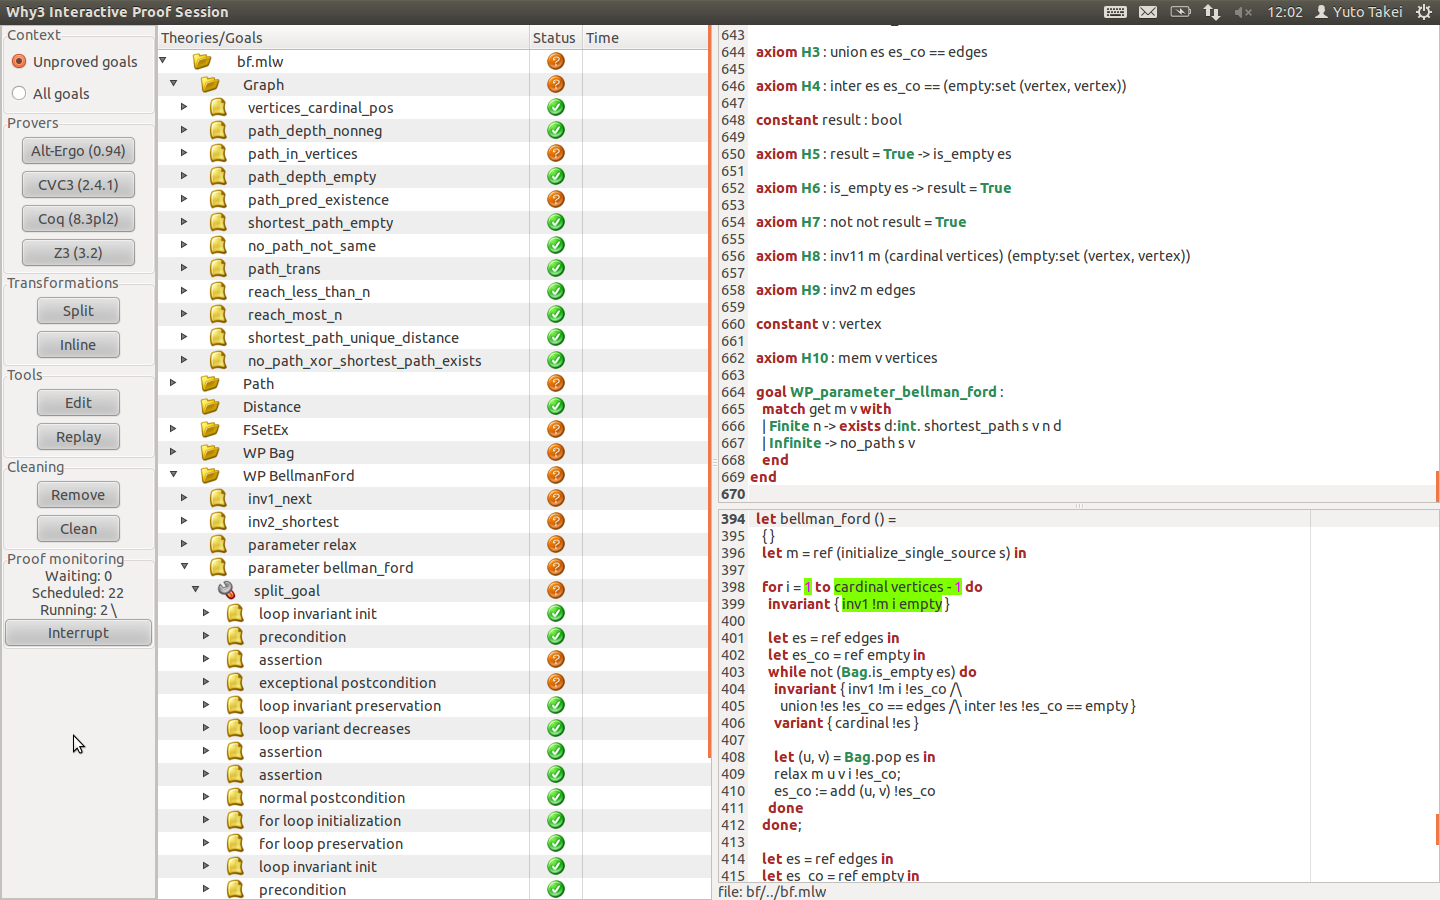
\includegraphics[width=\textwidth]{why3.png}
\caption{Graphical user interface of Why3}\label{fig:why3ide}
\end{figure}

I divided the correctness of the Bellman-Ford algorithm into following
four properties to be preserved.

\begin{enumerate}
\item The algorithm must terminate.
\item Non-reachable vertices from \texttt{s} must have infinity length
  after the termination.
\item Other vertices must have the length of the shortest path from
  \texttt{s} after the termination, if no negative length cycle exists
  in the graph.
\item If and only if there is at least one negative length cycle in
  the graph, the algorithm must terminate with exception.
\end{enumerate}

During the internship, I successfuly proved the first two properties,
which will be described in this report. The other two are left for the
future work.

\paragraph{Termination} First, we start by the termination property. Why3
requires loops and recursive functions to have an integral expression
as a variant. The expression should strictly descrease at each
iteration, and should stay positive except for the very last
iteration. This guarantees that the variant will finally converge to
zero in the finite number of steps, giving an upper bound for the
number of iterations.
 
\begin{algorithm}
\caption{Variants given for the loop termination}\label{lst:why3term}
\begin{why3}
let m = ref (initialize_single_source s) in
for i = 1 to cardinal vertices - 1 do
  let es = ref edges in
  while not (Bag.is_empty es) do
    variant { cardinal !es }
    let (u, v) = Bag.pop es in
    relax m u v
  done
done; (* code continues *)
\end{why3}
\end{algorithm}

For example, Line 1-6 in Algorithm \ref{alg:bf} are translated into
Why3 syntax as shown in Listing \ref{lst:why3term}. The inner
\texttt{while} loop got the number of edges to be processed as its
loop variant. It strictly descreases every time the iteration
proceeds. The outer \texttt{for} loop is more obvious and it is not
neccessary to add the redundant annotation.

In the same manner, we can add the variant for the loop at Line 7-11
in Algorithm \ref{alg:bf}. After giving the variants for loops, we
launch Why3 IDE to try prove the termination as illustrated in Figure
\ref{fig:why3term}.

\begin{figure}[h]\centering
\includegraphics[width=0.6\textwidth]{termination.png}
\caption{Proof session of algorithm termination}\label{fig:why3term}
\end{figure}

\paragraph{Non-reachable vertices} For next, we prove the property that the
vertices which have infinite length after algorithm termination must
be not reachable from \texttt{s}, i.e., no path exists from \texttt{s}
to them.

Generally speaking, users are expected to involve in giving
appropriate annotations in Why3 proof session because SMT solvers
cannot infer enough premises to prove the goal without them. The
annotations include invariants for loops, precondition and
postcondition for referring functions, and assertions at arbitrarily
point of execution.

In order to prove this property, we must note that the vertices which
can be reached by any paths with $d$ steps will be labeled with the
finite distance no later than $d$-th iteration of outer loop for
relaxation. Additionally relaxation of edges from vertices with finite
distance will let the destination vertices of such edges have the
finite distance as well. This shows that if a vertex $v$ with infinite
distance at $d$-th iteration after relaxation of some edges $E'
\subset E$, then there is no path from $s$ to $v$ with $d$ steps and
vertices $V'=\{u\in V\vert (u,v)\in E'\}$ have infinite distance.

The invariant in Why3 syntax is illustrated as in Listing
\ref{lst:why3inv}. \texttt{m}, \texttt{pass} and \texttt{via} in
parameters respectively represent the distant mapping at the moment,
the iteration count, and the edges that are already processed during
the current iteration.

\begin{algorithm}
\caption{Invariant for the property about non-reachable vertices}\label{lst:why3inv}
\begin{why3}
predicate inv (m: distmap) (pass: int) (via: set (vertex, vertex)) =
  forall v: vertex. mem v vertices ->
  match m[v] with
    | Finite n -> true
    | Infinite ->
      (forall d: int. 0 <= d < pass ->
        forall n: int. not (path s v n d)) /\
      (forall u: vertex. mem (u, v) via ->
        forall d: int. 0 <= d < pass ->
        forall n: int. not (path s u n d))
  end
\end{why3}
\end{algorithm}

\section{Discussions}


\section{Conclusion}

\pagestyle{empty}

\bibliographystyle{plain}
\bibliography{./biblio}

\end{document}
